

\section{Mapping Victims with academic datasets}\label{sec:mapping_victim}
This analysis seeks to bridge our recorded DDOS event data with insights derived from academic datasets, specifically those provided by Telescopes and Honeypots. Telescopes operate by analyzing backscattered traffic, indicative of attacks spoofing their source address to mimic that of the Telescopes' own address blocks. This detection method suggests that, despite our robust mitigation mechanisms, there is a nuanced possibility of overlap between the dates recorded by Telescopes and our event dataset. Such an overlap may either precede our event window, suggesting early detection and subsequent mitigation activation, or follow our event timeframe, possibly indicating an attack's resurgence post-mitigation.

Contrastingly, Honeypots offer a distinct perspective by actively participating in attack mechanisms, thereby aligning their data with DDOS events perhaps serendipitously. The presence of a Honeypot record during a DDOS event does not directly correlate with our mitigation processes due to their independent operation.

Building upon this foundation, our victim mapping effort leverages these academic datasets—enriched with dates and victim IP addresses from entities like Orion, UCSD, AmpPot, and Hopscotch—to correlate external attack indicators with our internal DDOS attack records. This correlation focuses on attack specifics such as duration (\texttt{startTime} to \texttt{endTime}), magnitude, types, and targeted victims, aiming to determine if academic data can preemptively signal potential threats to our clients. This is assessed across three critical junctures: before detection by our systems, during the transition to our protective measures, and following successful attack mitigation.

Our methodology unfolds in two phases. Initially, we extract our customers' IP address spaces from the academic datasets, filtering out irrelevant data to define a subset termed "customer IP space." Subsequently, we map these academic datasets' dates and victim IP addresses against our defined attack periods and the IP addresses associated with our customers' DDOS attack events. This meticulous mapping yields a refined dataset, "customer event IP," facilitating a targeted analysis of the interplay between academic insights and our DDOS event records.

Fig \ref{fig:addresssets} presents the relationships among our refined datasets. 

\begin{figure}[htbp]
    \centering
    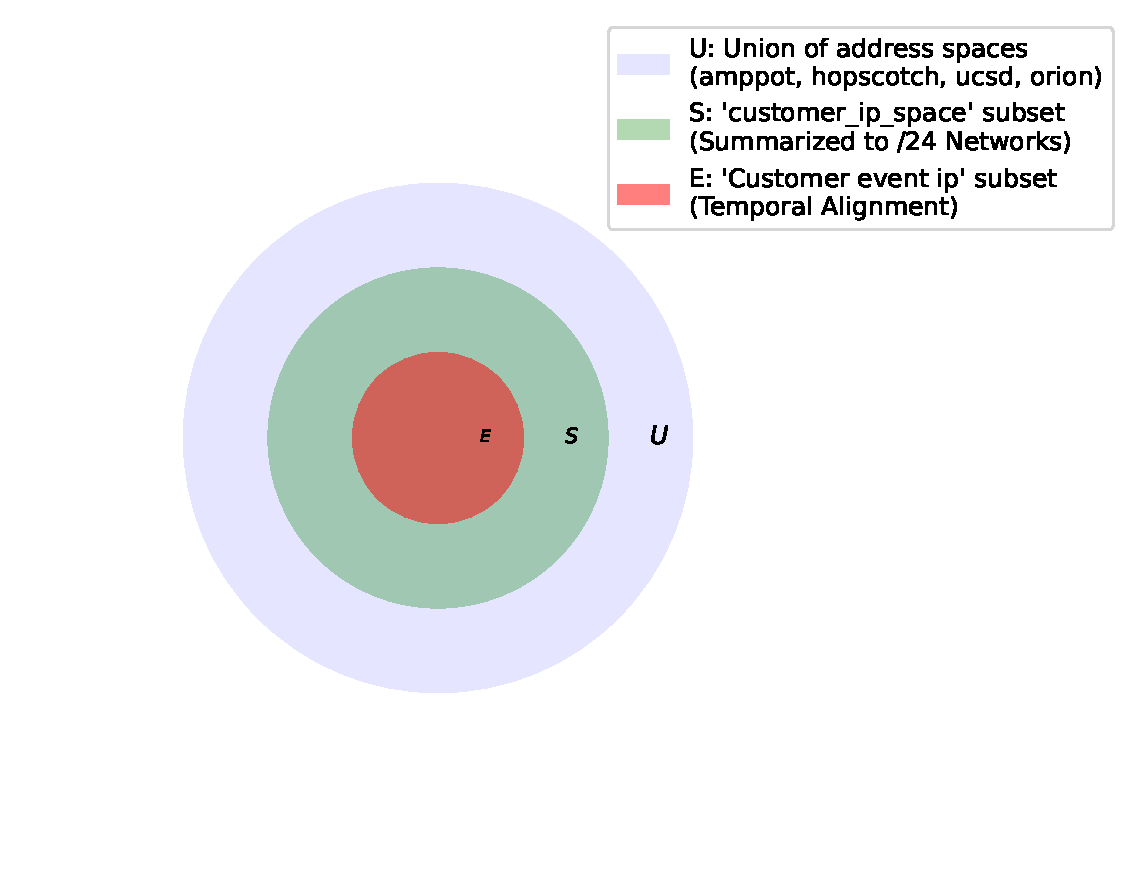
\includegraphics[scale=0.5]{graphs/sets.pdf}
    \caption{Address sets relationship}
    \label{fig:addresssets}
\end{figure}

\subsection{'Customer IP Space $S$' Definition}
Let $U$ represent the union of address spaces from the categories 'amppot', 'hopscotch', 'ucsd', and 'orion'. The 'customer\_ip\_space' condition identifies a subset of $U$, denoted as $S$, characterized by the following criteria:
\begin{enumerate}
    \item \textbf{Summarization to /24 Networks}: Each IP address in $S$ is summarized to a /24 Class C network, represented by the first three octets of the IP address, effectively transforming the address into a /24 network notation. 
    \item \textbf{Match with Summarized /24 Networks}: An address $s \in S$ is considered part of 'customer\_ip\_space' if its summarized /24 network matches with any summarized /24 network within $U$.
    \item The necessity for this summarization approach stems from the operational framework of our network protection strategy By receiving and propagating these prefixes (minimum /24 prefix for Internet reachability), we can redirect all inbound traffic destined for our customers from the Internet using Border Gateway Protocol (BGP). 
\end{enumerate}

\subsection{'Customer event ip $E$' Definition}
The 'Customer event ip' condition extends the identification of relevant IP addresses by incorporating temporal alignment with specific events. It represents a subset of 'customer\_ip\_space', denoted as $E$, with the following additional condition:

\begin{enumerate}
    \item \textbf{Temporal Alignment with Events}: For an address $e \in E$, not only must it satisfy the 'customer\_ip\_space' criteria, but it must also coincide with an event whose duration ($p$) matches a specified date ($d$). The event duration is defined by the start and end times of activity associated with the IP address. An event is considered to match if $d$ falls within this duration, indicating that the event occurred within the specified timeframe.
\end{enumerate}

\subsection{Analysis of 'Customer IP Space \(S\)'}
The refined dataset under analysis includes active customers who have reported DDOS attacks from January 1, 2019, to October 12, 2023. This dataset deliberately excludes those who have not reported any DDOS activities within this period, as well as customers who utilize non-network protection services, such as traffic redirection through DNS record management.

Included within this dataset are instances of attack traffic detected both prior to and subsequent to the initiation of our mitigation efforts. Before these efforts commence, data from both telescopes and honeypots contain records of attack activities directed at our customers. This initial state provides a comprehensive view of the attack landscape before any intervention.

After customers redirect their traffic to our platform and our mitigation measures become operational, the impact on attack traffic visibility varies by the nature of the monitoring systems. For darknet telescopes, the effect of our platform's attack traffic filtering leads to a significant reduction in backscattered traffic, effectively rendering these attacks invisible in the dataset. Conversely, when attacks originate from honeypots acting as DDOS reflectors, although our platform successfully filters the incoming attack traffic, the honeypots' ability to continuously send attack traffic means they can still document traffic and activities. 

The differential impact of our filtering mechanisms on these datasets leads to an expected discrepancy in recorded attack events between telescopes and honeypots. While honeypot setups may document a sustained or increased number of attack events due to their operational continuity, the telescope dataset is anticipated to show a reduced count as a direct consequence of our mitigation efforts. 

Fig. \ref{fig:customeripspace} show that AmpPot and Hopscotch collectively detected more than 50\% of attack events. This indicates a significant coverage and effectiveness in detecting DDOS attacks within the customer IP space managed by these honeypots. In contrast, Telescope UCSD and Orion reported lower detection rates, revealing around 29.3\% and 18.39\% of addresses, respectively.

\begin{figure}[htbp]
    \centering
    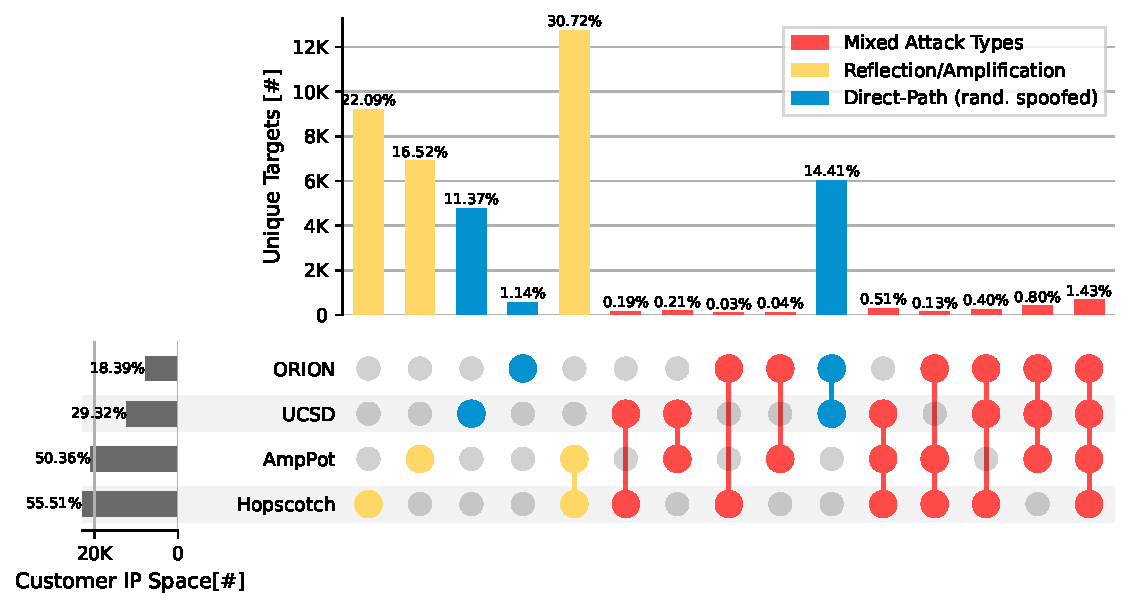
\includegraphics[scale=0.4]{graphs/space_no_event.pdf}
    \caption{Customer IP Space Analysis.}
    \label{fig:customeripspace}
\end{figure}


\subsection{Analysis of Customer Event IP \(E'\)}
The analysis of Customer Event IP \(E'\) is designed to enforce a more rigorous approach in identifying coincidences between the attacks detected by Telescopes and Honeypots and the attack events reported in our customer records. This entails a meticulous process where the 'Customer Event IP Datasets' must closely align victim IP addresses with the specific time periods of reported attacks.

We project that setups involving honeypots will uncover a higher frequency of coincidental events. This is attributed to their proactive role in engaging with and capturing malicious traffic, thus providing a rich dataset for analysis. On the other hand, observations from darknets are anticipated to present a lower occurrence of coincidental events. The passive nature of darknets, focused on the surveillance of unsolicited traffic across designated IP spaces, contributes to this expected discrepancy. The insights derived from this comparative analysis are invaluable, offering a deeper understanding of the threat environment confronting our customers and enabling the refinement of our defensive strategies accordingly.

Fig. \ref{fig:customereventip} This figure demonstrates that AmpPot's detection rate has risen to 61.13\%, while Hopscotch has recorded a 49.38\% detection rate. Such figures underscore their substantial reach and efficiency in identifying DDOS attacks within the customer event IP space. In comparison, Telescope UCSD and Orion have registered lower detection rates, decreasing to 26.48\% and 18.08\% of addresses, respectively.

\begin{figure}[htbp]
    \centering
    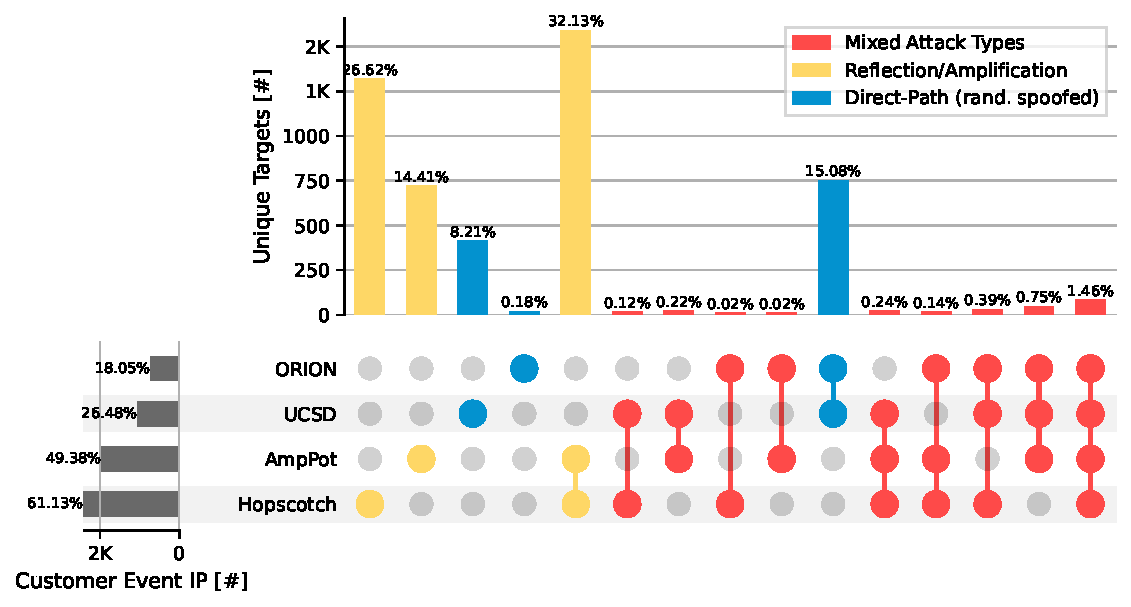
\includegraphics[scale=0.4]{graphs/space_event.pdf}
    \caption{Customer Event IP Analysis.}
    \label{fig:customereventip}
\end{figure}


Fig. \ref{fig:Mappedaddressanalysis} summarises the analysis of Customer IP Space, $S$ and Customer Event IP $E$.
\begin{figure*}[htbp]
    \centering
    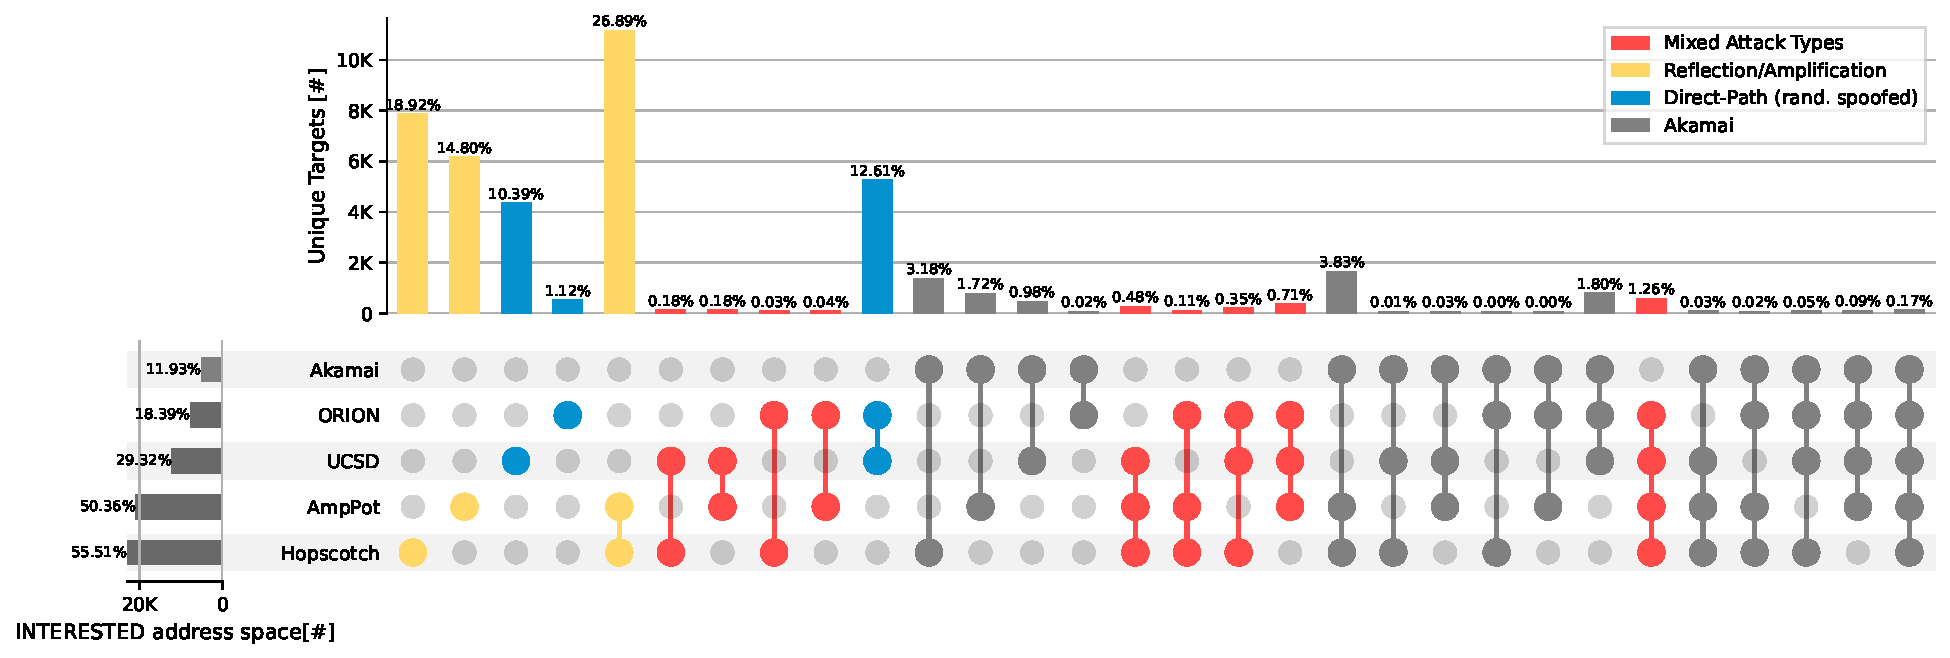
\includegraphics[scale=0.48]{graphs/noir3.pdf}
    \caption{Customer IP Space and event Analysis.}
    \label{fig:Mappedaddressanalysis}
\end{figure*}



\begin{figure}[htbp]
    \centering
    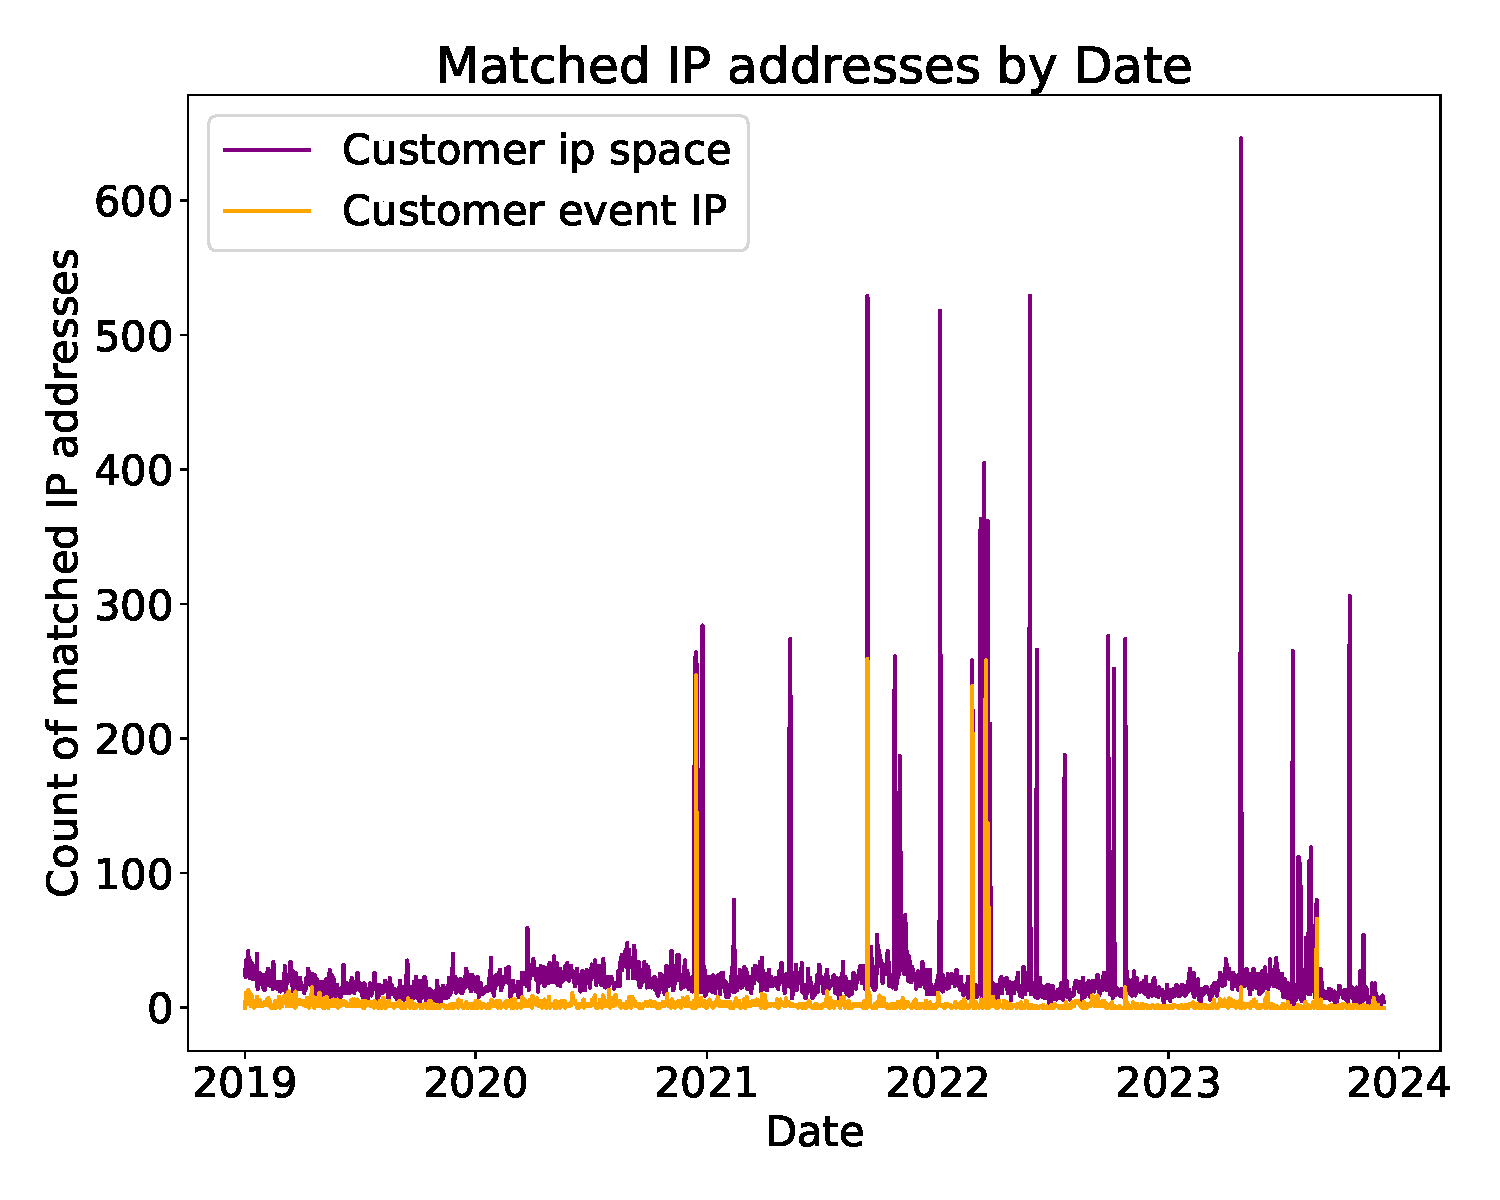
\includegraphics[scale=0.30]{graphs/matched_customer_graph.pdf}
    \caption{Mapping customer ip space and event.}
    \label{fig:mappedcustomergraph}
\end{figure}


\subsection{Special Attack Incidents Analysis}\label{sec:attackeventsfromcustomeripspace}
The observed spike in Fig. \ref{fig:mappedcustomergraph} shows an abrupt jump in the number of victim (target) addresses on a particular date, which indicates that our customer prefix(es) in the Customer IP Space dataset may under horizontal attack. Normally, we observe the number of target addresses to be less than 50 daily, as indicated in Fig. \ref{fig:akamai_spikes}, which shows the distribution of the number of target addresses grouped by victim /24 prefix and date of attack. This observation is particularly interesting as mentioned in our company blogs \cite{Birchard2022DDoS}. We are seeing an increasing trend of horizontal attacks, referring to simultaneous DDoS attacks aimed at multiple, unrelated targets (which is why they’re sometimes called carpet bomb attacks). Instead of prioritizing a single high-value target, the attacker selects multiple targets in order to distribute the attack, making it more challenging for security teams to mitigate and maximizing the possibility of widespread disruption. 

% Fig. visualizes the count of matched IP addresses over time, distinguishing between "Customer IP Space" and "Customer Event IP". It shows spikes indicating significant events: (A) a large number of targets detected from the Customer IP Space $S$ by telescopes/honeypots and (B) a large number of targets from Customer Events records by the DPS coincided with the telescopes/honeypots, address space $E$.
% Amppot, Hopscotch, UCSD, and Orion

\subsection{Spikes Detected by Academic datasets}
Table \ref{table:spikes_data} outlines the detection of significant attack instances confirmed with our reported events, illustrating that some malicious activities are observable through network telescopes, while others are unveiled by honeypot infrastructures.
\begin{itemize}
\item \textbf{Network Telescopes:} Instruments like UCSD and Orion are crucial for identifying spoofed assault attempts on IP ranges, evidenced by anomalous backscatter signals. These incidents predominantly occur in two situations:
\begin{enumerate}
\item When an entity engages DDoS Protection Services for imminent threat mitigation.
\item During the initial phase before the full implementation of mitigation strategies.
\end{enumerate}
\item \textbf{Honeypots:} Tools such as Amppot and Hopscotch are effective in detecting both straightforward and complex attacks, maintaining vigilance over entire targeted IP segments. 
\end{itemize}

Telescope detections often involve straightforward attack mechanisms like UDP, SYN, and NTP floods, as well as TCP irregularities, leveraging the telescope's IP space as spoofed origins.

In contrast, honeypots reveal the intricacies of amplification and reflection attacks, such as those involving DNS and NTP, demonstrating their capability to expose and analyze these more complex attack vectors.








\begin{table*}[htbp]
    \centering
    \caption{Matched IP counts showed as spikes in Fig \ref{fig:mappedcustomergraph}}
    \begin{tabular}{|l|l|r|r|r|r|r|}
    \hline
    \textbf{Date} & \textbf{Victim Subnet} & \textbf{Amppot} & \textbf{Hopscotch} & \textbf{UCSD} & \textbf{Orion} & \textbf{Akamai} \\
    \hline
    2020-12-15 & Subnet A & 83 & 246 & 0 & 0 & 246 \\
    2021-09-12 & Subnet B & 0 & 0 & 256 & 256 & 256 \\
    2022-02-25 & Subnet C & 1 & 1 & 239 & 0 & 239 \\
    2022-03-18 & Subnet D & 1 & 256 & 1 & 1 & 256 \\
    2022-03-22 & Subnet D & 0 & 135 & 1 & 1 & 135 \\
    2023-08-24 & Subnet E & 0 & 0 & 66 & 66 & 66 \\
    \hline
    \end{tabular}
    \label{table:spikes_data}
    \end{table*}


The information in Table \ref{table:spikes_data} correlates directly with the DDoS events we've monitored, specifically through the sudden increases observed within our Customer Event IP dataset. This dataset pinpoints IP addresses within our customers' network prefixes that have been flagged by either the telescope or honeypot monitoring systems. The term "Customer Event IP" is particularly attributed to those IP addresses that are not only detected in the monitoring datasets but also align with the wider time windows marked by the \texttt{startTime} and \texttt{endTime} of observed DDoS incidents. It's important to note that this alignment does not rely on the precise timing (hour, minute, and second) due to the monitoring data's lack of such detailed timestamps. Instead, the matching process is based on the assumption that each date recorded represents the entire 24-hour period from midnight to midnight, ensuring that the correlation considers the full day's potential for attack activity.


\begin{figure*}[htbp]
    \centering
    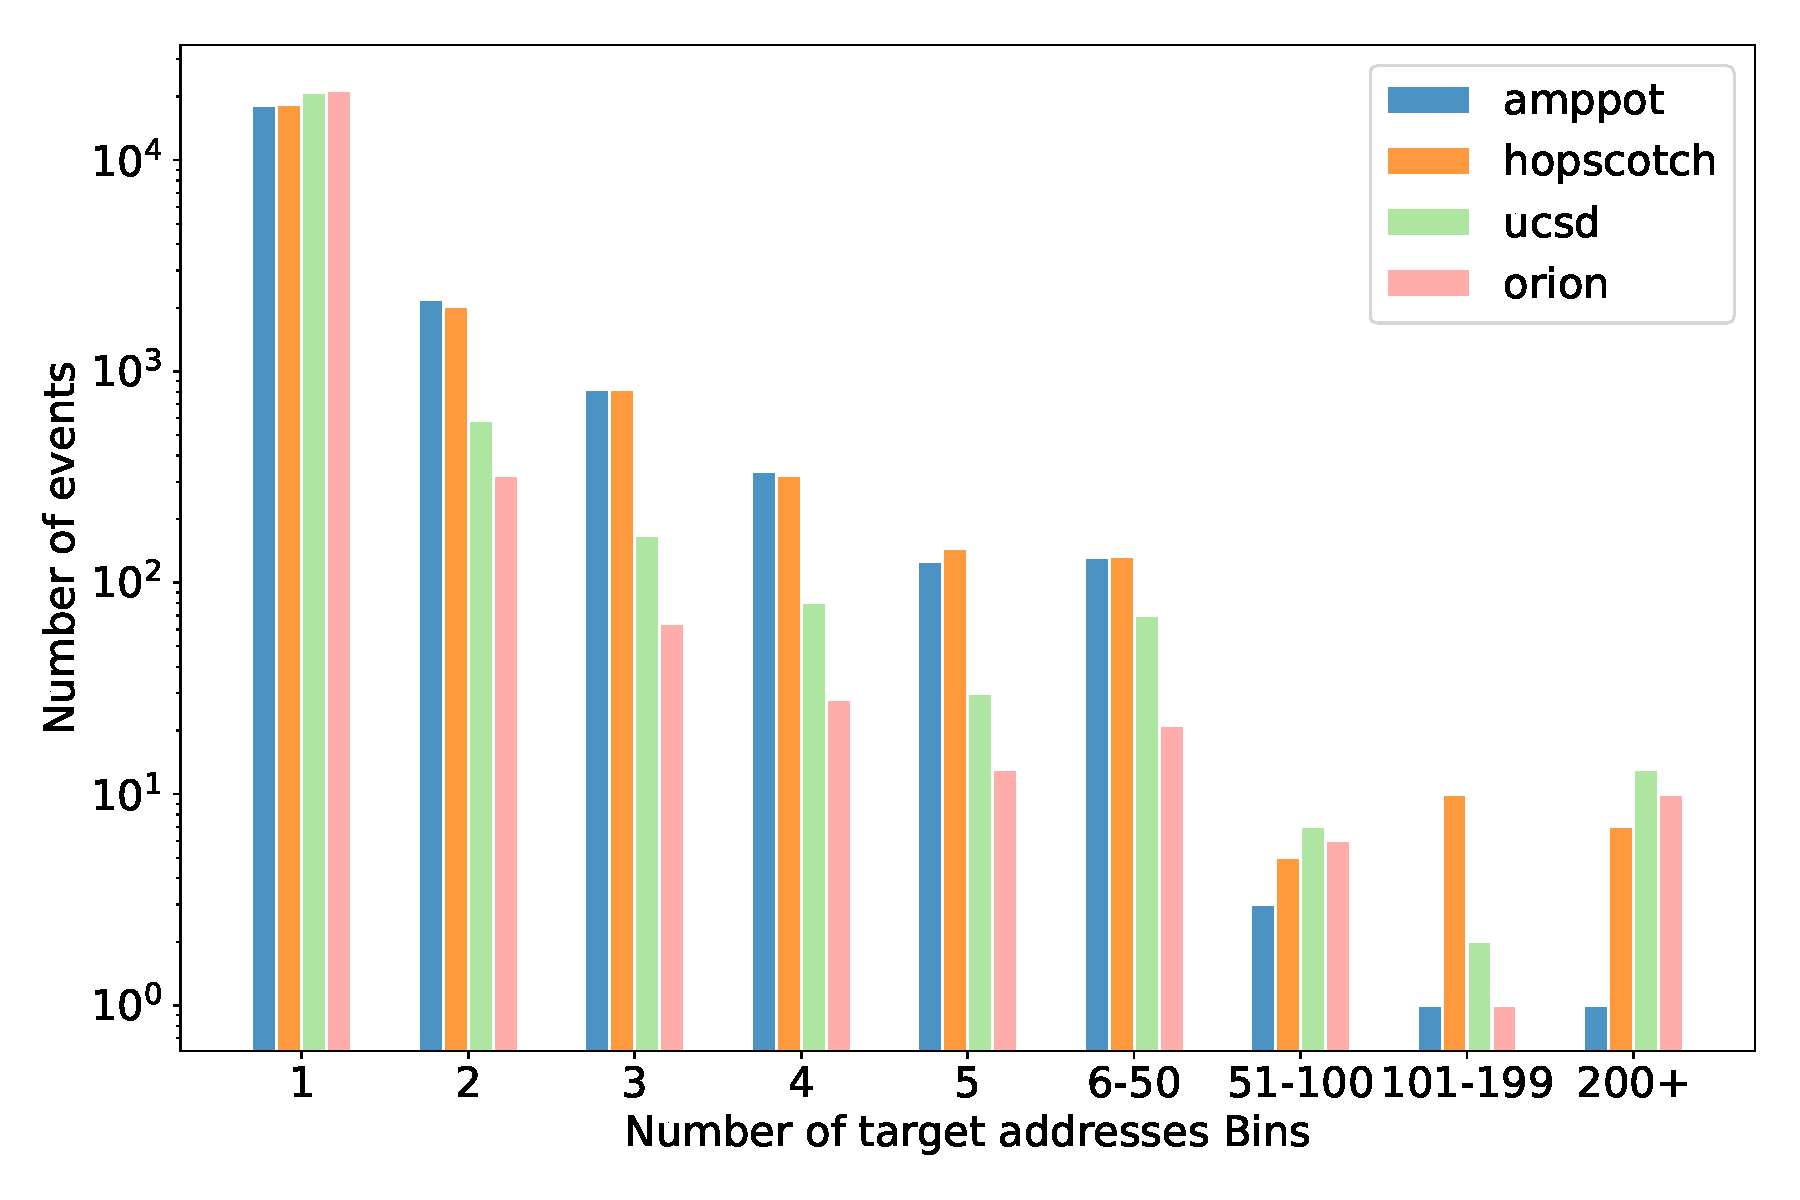
\includegraphics[scale=0.48]{graphs/space_bin_log.pdf}
    \caption{Distribution of Number of victim ip grouped by date and /24 prefixes.}
    \label{fig:akamai_spikes}
\end{figure*}




% \section{Mapping victims with Telescopes and Honeypot}\label{sec:mapping_victim}
% This analysis establish a relationship between our recorded DDOS event data and the Telescopes and  Honeypots datasets. It specifically focuses on aligning full-day dates, spanning from midnight to the end of the day, with our defined intervals of DDOS events, as marked by startTime and endTime. 
% In Telescopes' operational design, attacks are detected by analyzing backscattered traffic. This traffic typically results from attack traffic that spoofs its source address to resemble that of the Telescopes' address blocks. Based on this detection method, we can anticipate two primary scenarios:
% Due to our mitigation mechanisms, there is only a slim chance that the date recorded by Telescopes will coincide with our event dataset. If Telescopes record a date that precedes the startTime and endTime of a DDOS event, it might be indicative of an attack being detected early by the Telescopes. Following this early detection, mitigation measures might be activated within the DDOS event window to address the attack. On the other hand, if a date recorded by Telescopes falls after the DDOS event timeframe, it could imply a re-emergence of the attack, occurring after the mitigation measures detailed in the DDOS event data.
% The Honeypots dataset, however, provides a contrasting perspective. Unlike Telescopes, Honeypots are not just detection tools; they actively participate in attack mechanisms. As such, their data might align with DDOS events by coincidence. The occurrence of a Honeypot record during a DDOS event does not inherently suggest a direct link with the event's mitigation processes, as Honeypots operate independently of these countermeasures.

% The aim of victim mapping revolves around leveraging academic datasets to enhance our understanding and response to DDOS attacks affecting our clients. These datasets, provided by institutions such as Orion and UCSD, as well as operations like AmpPot and Hopscotch, include precise data points such as dates and victim IP addresses. Utilizing this information, we endeavor to correlate these external data points with our internal records of DDOS attacks---marked by specifics such as attack duration (\texttt{startTime} to \texttt{endTime}), attack magnitude, types, and targeted victims. Our objective is to ascertain whether these academic datasets offer a viable means to preemptively identify potential threats to our customers---be it prior to our detection systems picking up on the attack, during the transition of attack handling to our protective measures, or post the successful mitigation of the DDOS attack through our platform.

% In the initial phase of our methodology, we sift through the academic datasets to extract our customers' IP address spaces---this step helps in filtering out data unrelated to our platform or clientele, thereby defining our first subset of data, termed as ``customer IP space.''

% Following this, we proceed to the second phase where we map the academic datasets' dates and victim IP addresses against our internal records' defined attack periods (\texttt{startTime} and \texttt{endTime}), alongside the IP addresses associated with our customers' DDOS attack events. This mapping process culminates in the creation of a refined dataset, designated as ``customer event IP,'' which enables a focused analysis of the correlation between academic findings and our own DDOS event records.
